\documentclass[12pt]{article}
\usepackage[francais]{babel}
\usepackage[T1]{fontenc}
\usepackage[utf8]{inputenc}
\usepackage[top=3cm, bottom=2cm, left=2cm, right=2cm]{geometry}
\usepackage[babel]{csquotes}
\usepackage[normalem]{ulem}
\usepackage{graphicx}
\usepackage{eurosym}
\usepackage{tabularx}
\setlength{\headsep}{0.5in}
\renewcommand{\baselinestretch}{1.35}
\setlength{\footnotesep}{0.4cm}
\setlength{\skip\footins}{1cm}
\MakeAutoQuote{«}{»}
\pagestyle{headings}
\graphicspath{{img/}}

\begin{document}

\pagenumbering{gobble}
\begin{titlepage}

	\flushleft{
		\textit{
			17 Mai 2014
		}
	}

	\flushright {
		GONZALEZ Julien \emph{(gonzal\_j)} \\
		GUYOT DE CAMY Matthieu \emph{(guyot-\_m)} \\
		CAVALIÉ Quentin \emph{(cavali\_q)} \\
		DUMONT Matthieu \emph{(dumont\_h)} \\
		\textbf{EPITA 2015}
	}

	\begin{center}
		\vspace*{\stretch{1}}

		{
			\Huge
				\textsc{
					\textbf{
						Projet de Fin d'Études en Entreprise \\
					}
				}
		}
		{
			\LARGE
				\textsc{
					\textbf{
						Suivi n\degree 2 \\
					}
				}
		}

		{
				
\includegraphics[width=100px]{jellynote.png}\hspace{3cm}
\includegraphics[height=50px]{epita.jpg}\\
				[1cm]
		}

		\textbf{
			\textit {
				Génération de partition en temps-réel par microphone.\\
				[1cm]
			}
		}
		\vspace*{\stretch{1}}
	\end{center}
	\flushright {
		\textbf{Dates du projet:} \textit{de Mai 2014 à Janvier 2015}
	}
\end{titlepage}

\pagenumbering{arabic}

\newpage
\tableofcontents

\newpage
\clearpage

\section{Introduction}

Ce Projet de Fin d'Études en Entreprise sera réalisé avec l'entreprise Jellynote, jeune start-up connaissant une très forte croissance, specialisée dans l'apport de contenu musical pour les gens débutants ou souhaitant améliorer leur pratique dans un instrument de musique.\\

Notre projet consiste en outil de génération à la volée de partitions. Celui-ci pourrait s'interfacer directement avec l'application client de Jellynote et leur permettre de proposer un outil supplémentaire à leurs utilisateurs.\\

Par ailleurs, notre travail s'axerait sur la proposition d'une librairie open-source de génération de partitions, permettant d'ouvrir notre application destinée à des professionnels à un éventail bien plus large d'utilisateurs.\\

Nous tenons enfin à remercier le professeur Reda Dehak pour nous avoir mis en relation avec cette entreprise, donnant ainsi à ce projet une dimension professionnelle et nous offrant ainsi un cadre propice au développement d'une telle application.


\newpage
\section{L'entreprise}
Jellynote est une plate-forme pour les musiciens en ligne. On y trouve tous les outils pour apprendre et jouer de la musique: des partitions, des tablatures, des vidéos d’interprétations etc. Jellynote est une jeune start-up qui a aujourd’hui presque 2 ans. Elle fut créée le 1er juin 2012 par Arthur Lenoir, Baptiste Poirier et Adrien Cognée.\\

Jellynote a pour vocation de faciliter la pratique de la musique. Le secteur de la pratique musicale peut être divisé en trois catégories : les débutants, qui ont des besoins pédagogiques très spécifiques, les amateurs qui ont essentiellement besoin de ressources variées et les musiciens expérimentés qui n’ont soit besoin de rien, soit ont besoin d’un contenu de très haute qualité.\\

L'aspect de la plate-forme Jellynote qui a le plus de similarités avec notre projet de PFEE et qui nous a poussé à nous associer avec eux est le système de reconnaissance d’accords et de notes en ligne tournant en temps réel. Le but de ce système est de vérifier, par le biais d’un microphone, ce que l’utilisateur joue devant son écran. L'utilisateur peut ainsi jouer de son instrument devant son ordinateur afin de valider ou non les notes.

\newpage
\section{Cahier des charges}

Notre projet est dans la lignée de ce qui est déjà réalisé par Jellynote, mais comporte des différences notables. Il s’agit de prendre un signal sonore provenant d’un enregistrement de guitare, et de le traiter pour ensuite générer la partition correspondante.\\

Les développeurs de Jellynote s’étaient déjà penchés sur une même problématique, mais sans la mener à bout par faute de temps. Il s’agit pour nous d’amener l’idée à maturation. L’objectif principal n’est donc pas d’intégrer le service dans Jellynote, même si l’entreprise se réserve le droit de l’intégrer par la suite.\\


Nous pensions au départ partir sur une détection automatique du tempo et de la signature rythmique, mais après des discussions avec notre contact à Jellynote, il s'est avéré que cela posait trop de problèmes techniques. Nous avons donc décidé de laisser l'utilisateur entrer lui-même le tempo et la signature rythmique désirée, à la manière des autres applications Jellynote.\\

Un autre aspect que nous avons changé par rapport à notre idée originelle est sur le traitement en temps-réel de l'entrée micro. Nous avions au départ prévu d'analyser des fichiers audio pré-enregistrés, mais le temps-réel est plus en phase avec l'environnement Jellynote.\\

Les discussions avec l’équipe de Jellynote nous ont confortées dans la faisabilité de notre projet, et les connaissances des développeurs dans ce domaine nous rassurent quant au lancement du projet et à l’aide qu’ils nous apporteront en cas de blocage.\\


Ce projet n’est pas destiné à l’attention d’un public particulier. C’est avant tout l’aspect technique qui est primordial, et c’est l’équipe de Jellynote qui nous notifiera de la possibilité de l’intégrer à terme dans l’environnement Jellynote.\\

\newpage
\subsection{Livrables}
Le projet comporte une partie principale que nous nous engageons à livrer. Il sera ensuite éventuellement composé de modules supplémentaires que nous pourrons greffer au logiciel afin d’en enrichir ses fonctionnalités.\\

\subsubsection{Livrable obligatoire}

Le livrable obligatoire se compose d’un logiciel comportant une interface graphique simple permettant de :\\
\begin{itemize}
\item Paramétrer le tempo et la signature rythmique.
\item Lancer l'enregistrement du son.
\item Visionner la partition qui s'affiche au fur et à mesure que l'enregistrement se fait.\\
L’équipe Jellynote dispose déjà des outils nécessaires pour afficher des partitions, et nous pourrons donc nous en servir pour gérer l'affichage.
\end{itemize}

\subsubsection{Livrables optionnels}

Voici les fonctionnalités qui seront ajoutées au livrable si le temps nous le permet :
\begin{itemize}
\item Gestion d’autres instruments: piano, basse…
\item Gestion de rythmes plus complexes (7/8, 9/8, 5/4…)
\item Gestion des divisions artificielles du temps (quintolets, septolets…)
\end{itemize}

\newpage
\section{Aspects fonctionnels}

\subsection{Diagramme fonctionnel}
\vspace{1cm}
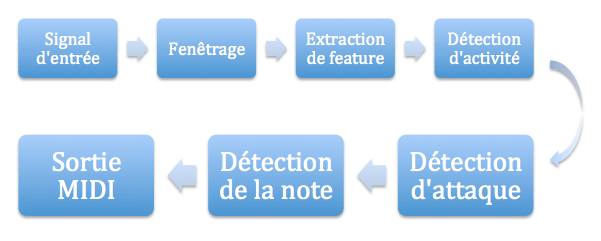
\includegraphics[height=150px]{diagfunc.png}

\newpage
\subsection{Les risques}

Les risques liés à ce projet sont uniquement logiciels, puisqu’il n’y a pas d’attentes au niveau de l’infrastructure ou de la sécurité.\\

Le risque principal réside dans la bonne \textbf{reconnaissance des accords et du tempo}. La reconnaissance de notes individuelles ne devrait pas poser de gros problèmes, en revanche les combinaisons de notes pour former des accords posent des problèmes techniques plus poussés, de même que l'affichage en temps-réel des partitions. Ayant appris tardivement ce changement, nous ne pouvons mesurer à quel point le temps-réel pourra être respecté (ie. si il y aura un léger retard, et à quel point). \\

Les risques secondaires sont ceux-ci :
\begin{itemize}
\item \textbf{Reconnaissance des accords} : Les harmoniques peuvent être difficiles à différencier (ex: reconnaître un C5 au lieu d’un C4). Nous pourrons mitiger ce risque grâce à l’expérience des développeurs de Jellynote dans ce domaine, qui seront à même de nous guider vers des solutions appropriées.
\item \textbf{Fausses notes} : Les fausses notes pourront poser des problèmes pour des raisons évidentes. Il faudra alors les détecter pour ensuite les corriger, enlever, ou encore signaler à l’utilisateur qu’elles sont fausses.
\end{itemize}

\subsection{Relation avec l'entreprise}

L’équipe de Jellynote étant bien plus expérimentée que nous dans les domaines abordés, nous comptons travailler le plus possible avec des retours fréquents de leur part.\\

Nous comptons pour cela faire une réunion une fois par mois (par mail ou par Skype), afin de leur relater de notre avancement, et leur remonter les éventuels problèmes rencontrés afin de solliciter leur aide si le besoin s’en fait ressentir.\\

Ces réunions nous permettront également de jauger la possibilité d’intégrer notre projet à Jellynote.

\newpage
\section{Aspects techniques}
\subsection{Langage utilisé}

Le langage utilisé pour implémenter le projet sera principalement voire exclusivement du C++. Cependant, en fonction des possibilités offertes par certaines bibliothèques de fonctions, il est possible que certains modules soient implémentés dans d’autres langages. Le choix du C++ est décidé par la volonté de Jellynote de porter ses sources vers ce langage ainsi que par la puissance de modélisation que ce dernier offre.\\

\subsection{Description globale de l’application}

L’entrée du programme sera un flux vidéo, directement enregistré via une entrée micro par l'utilisateur. La sortie sera une partition en format MIDI, qui sera affichable dans le logiciel.\\

Le projet ne pourra directement aboutir en quelques semaines à son objectif final. Il devra passer par des phases intermédiaires admettant un niveau de complexité et de performance fonctionnelle et technique croissant. Ceci permettra la mise en place de sessions de tests sur les composants techniques de l’application ainsi que la validation de ces derniers.\\

Ces avancées se réaliseront à travers plusieurs niveaux de performance que les blocs de traitement du signal et de génération de partition atteindront par paire. En effet, une fonctionnalité nécessitera un module pouvant assurer l’extraction des données utiles à partir de la bande son analysée ainsi qu’un autre capable de les traiter pour pouvoir produire la sortie voulue. L’absence d’un de ses deux composants sera bloquante. C’est pourquoi nous avancerons par paliers sur les deux modules de manière simultanées. \\

L’ensemble du domaine musical sera décrit en utilisant la notation américaine standard en solfège. La gamme de référence sera la gamme tempérée. \\

\newpage
\section{Les paliers}

Les paliers décris ci-après ne prendront en compte que des morceaux jouées par une guitare unique à son clair et sans effets sonores (overdrive, phaser, flanger, chorus, delay etc). À moins d’une mention spécifiant le contraire, ce qui est requis à un palier, l’est pour les paliers suivants.\\

Ces étapes sont données à titre indicatif d’avancement et pourront subir de légères modifications en cas d’avancement ou de retard sur la guideline du planning. Évidement, le module de génération de partition et d’heuristique dépendant directement des capacités de traitement du signal de l’application, les contraintes exprimées sur la partie traitement du signal à chaque palier s’étendent sur la seconde section également.\\

Aussi, si on demande à un palier que le module de traitement du signal puisse gérer au maximum un accord de trois notes, il ne sera pas demandé de générer une partition comportant des accords de plus de trois notes.\\

Enfin, il est à noter que seuls les trois premiers paliers correspondent au livrable obligatoire. Les deux autres palies correspondent à des objectifs ultimes au niveau de l'application mais ne doivent pas être considérés comme étant les résultats attendus.

\newpage
\subsection{Palier 1}

Le premier palier aura comme objectif la mise en place des éléments de bases du projet ainsi que la communication entre le composant chargé de traiter le signal et celui chargé de générer la partition.\\

\subsubsection{Traitement du signal}

Le module doit pouvoir détecter la présence de notes ainsi que leur attaque dans le fichier son fourni et les différencier ayant comme référence la gamme tempérée. Les notes superposées ne sont pas à gérer. La précision sur la longueur des notes n'est pas requise et l’octave n’est pas demandée.

\subsubsection{Génération de partition}

Le module doit placer ces notes sur une partition à un tempo de 60 bpm (1 battement par seconde). Les notes doivent être disposées en terme de rythme sur la partition de la même manières qu'elles le sont dans le fichier son.

\newpage
\subsection{Palier 2}

Ce palier constituera l’entrée en matière en terme de technique, le précédent faisant office de mise en place de l’environnement de projet. \\

\subsubsection{Traitement du signal}

Le module doit détecter la longueur des notes jouées avec une tolérance +/- 1/2 seconde. L’octave de la note doit également être reconnue. ex : Un C4 est différent d’un C5. Le module doit pouvoir analyser les accords superposant jusqu’à 3 notes distinctes.\\

\textbf{N.B.} : Des notes X et Y sont distinctes si leur positions sur la gamme ou leur octaves diffèrent.

\subsubsection{Génération de partition}

Le module peut détecter le tempo d’un morceau en 4/4. Il ajuste les longueurs réelles en secondes des notes pour les exprimer en terme de rythme. Les divisions artificielles de temps ne sont pas à gérer. Il n’est pas assurer que les mesures soient toutes parfaitement remplies. Les silences ne sont pas gérés.

\newpage
\subsection{Palier 3}

Le présent palier représente l’accomplissement de la majeure partie des fonctionnalités.\\

\subsubsection{Traitement du signal}

Les différentes phases d’une note (attaque, decay, sustain et release) doivent être détectées. Cette détection nous permettra de détecter la longueur des notes avec précision.\\

Par ailleurs, nous devons détecter les accords. La difficulté consiste à détecter les différentes phases décrites précédemment pour chacune des notes et arriver à déterminer qu'elles appartiennent toutes au même accord.

\subsubsection{Génération de partition}

Nous nous attaquons à plusieurs gros chantiers :

\begin{itemize}
\item La détection de la gamme du morceau est gérée
\item Les dièses et bémols à l’armure sont définis
\item Les silences sont gérés
\item Le morceau est découpé en mesures
\item Les mesures sont toutes correctement remplies\\
\end{itemize}

Pour chacun de ces élements, nous nous basons quand même sur une simplicité du morceau assez importante. Nous ne gérerons pas des mesures originales et resterons sur des accords simples.

\newpage
\subsection{Palier 4}

Dans ce palier, nous nous attaquons à la détection d'accords plus complexes, et à la détection des mesures.\\

\subsubsection{Traitement du signal}

Nous nous fixons comme ojectif d'être capable de détecter jusqu'à 7 notes jouées en simultané.

\subsubsection{Génération de partition}

Nous désirons être capable de détécter les mesures, même originales, et éventuellement les changements de mesures.\\

Par ailleurs, le fichier MIDI en sortie peut comporter des divisions exceptionnelles de temps telles que les triolets et les sextolets.

\newpage
\subsection{Palier 5}

Ce dernier palier décrit les objectifs ultimes que nous nous fixons pour notre outil. \\

Nous nous lançons dans la reconnaissance d'effets.

\subsubsection{Traitement du signal}

Voici les différents effets que nous nous efforcerons de détecter :
\begin{itemize}
\item Le jeu legato
\item Le palm muting
\item Bends
\item Slides
\item Vibrato
\end{itemize}

\subsubsection{Génération de partition}

Différents objectifs ici :

\begin{itemize}
\item Le module doit calculer le tempo de morceaux en 3/4
\item Le "laisser sonner" est différencié de la longueur des notes
\item Le legato est géré ainsi que les bends, les slides et les vibratos
\item Le palm muting est géré
\end{itemize}

\newpage
\section{Tests}

\subsection{Test de qualité des partitions}
On utilise un fichier MIDI pour générer un fichier son, qu’on envoie ensuite dans notre programme. La partition de sortie est alors comparée au fichier MIDI d’entrée pour voir si le programme a correctement interprété le fichier audio.\\

\subsection{Test de robustesse}
Tester le logiciel avec des fichiers très lourds.

\subsection{Tests de complexité}
Effectuer de nombreux tests automatiques avec des séquences de plus en plus complexes (Accords, demi-croches, etc.)

\subsection{Tests manuels}
Beaucoup des fonctionnalités sont difficilement testables automatiquement, notamment au niveau des parties plus techniques du jeu de guitare. Il faut donc attentivement tester toutes les parties décrites dans les spécifications techniques.

\newpage
\section{Conclusion}

\end{document}